% !TEX TS-program = xelatex
% !TEX encoding = UTF-8 Unicode
% -*- coding: UTF-8; -*-
% vim: set fenc=utf-8

%%%%%%%%%%%%%%%%%%%%%%%%%%%%%%%%%%%%%%%%%%%%%%%%%%%%%%%%%%%%%%%%%
%% Thesis.tex
%% <https://github.com/zachscrivena/simple-thesis-dissertation>
%% This is free and unencumbered software released into the
%% public domain; see <http://unlicense.org> for details.
%%%%%%%%%%%%%%%%%%%%%%%%%%%%%%%%%%%%%%%%%%%%%%%%%%%%%%%%%%%%%%%%%

% See "README.md" for instructions on compiling this document.

\documentclass[letterpaper,nonstopmode]{simplethesisdissertation}

% Class options:
% a4paper, letterpaper, nonstopmode, draftmode.

%%%%%%%%%%%%%%%%%%%%%%%%%%%%%%%%%%%%%%%%%%%%%%%%%%%%%%%%%%%%%%%%%
%% PREAMBLE.
%%%%%%%%%%%%%%%%%%%%%%%%%%%%%%%%%%%%%%%%%%%%%%%%%%%%%%%%%%%%%%%%%

\usepackage{float}  % force figures into section

%\usepackage{hyperref}


\usepackage{geometry}
\geometry{a4paper, right=25mm, left=25mm, top=25mm, bottom=20mm}
%\usepackage[top=2cm,bottom=4cm,left=1.5cm,right=3cm]{geometry}
%\usepackage[utf8]{inputenc} % Required for inputting international characters
%\usepackage[T1]{fontenc} % Output font encoding for international characters
%\usepackage{palatino} % Use the Palatino font by default
\linespread{1.5}  % line spacing

% Document properties.
\def\DocumentTitle{Deep Neural Networks for predicting molecular properties}
\def\AuthorName{Raphael Peer}

% PDF settings and properties.
\hypersetup{
pdftitle={\DocumentTitle},
pdfauthor={\AuthorName},
pdfsubject={Master's Thesis, University of Salzburg},
pdfcreator={XeLaTeX},
pdfproducer={},
pdfkeywords={},
unicode=true,
pdfstartview=FitH,
pdfpagelayout=OneColumn,
pdfpagemode=UseOutlines,
hidelinks,
breaklinks,
bookmarksnumbered}

% Accent colors.
\definecolor{AccentOne}{RGB}{0,68,186} % blue

% Macros:
\DeclareMathOperator*{\argmax}{arg\,max}
\DeclareMathOperator*{\argmin}{arg\,min}
\renewcommand{\binom}[2]{\left(\genfrac{}{}{0pt}{}{#1}{#2}\right)}
\newcommand{\ceil}[1]{{\left\lceil{#1}\right\rceil}}
%\newcommand{\ffrac}[2]{{\nicefrac{#1}{#2}}}
%\newcommand{\fffrac}[2]{{\left.{#1}\middle/{#2}\right.}}
\newcommand{\floor}[1]{{\left\lfloor{#1}\right\rfloor}}
\DeclareMathOperator{\lcm}{lcm}
\newcommand{\ZZ}{{\mathbb{Z}}}

%%%%%%%%%%%%%%%%%%%%%%%%%%%%%%%%%%%%%%%%%%%%%%%%%%%%%%%%%%%%%%%%%
%% ACTUAL DOCUMENT.
%%%%%%%%%%%%%%%%%%%%%%%%%%%%%%%%%%%%%%%%%%%%%%%%%%%%%%%%%%%%%%%%%

\begin{document}


% Use Roman numerals (i, ii, iii, etc.) for page numbers in the front matter.
\pagenumbering{roman}

%%%%%%%%%%%%%%%%%%%%%%%%%%%%%%%%%%%%%%%%%%%%%%%%%%%%%%%%%%%%%%%%%
%% TITLE PAGE.
%%%%%%%%%%%%%%%%%%%%%%%%%%%%%%%%%%%%%%%%%%%%%%%%%%%%%%%%%%%%%%%%%

% No headers or footers on the title page.
\thispagestyle{empty}

\begingroup
\centering
\setstretch{1.0}
~
\\[1em]
\sffamily\bfseries\fontsize{26}{31.2}\selectfont
\DocumentTitle
%\\
%Use Manual Line Breaks If Necessary
\\[0.4in]
\normalfont\large
%Thesis by
%\\[0.25em]
\sffamily\bfseries\Large
\AuthorName
%\\[0.4in]
%\normalfont\normalsize
%In Partial Fulfillment of the Requirements
%\\[0.5em]
%for the Degree of
%\\[0.5em]
%Doctor of Philosophy
%\\[0.5em]
%in
%\\[0.5em]
%Electrical Engineering and Computer Science
\vfill
%\includegraphics[height=1.8in]{Figure-SchoolLogo}
%\\[1.5em]
University of Salzburg
\\[0.5em]
Salzburg, Austria
\\[1.5em]
2020
\par
\endgroup

\clearpage

%%%%%%%%%%%%%%%%%%%%%%%%%%%%%%%%%%%%%%%%%%%%%%%%%%%%%%%%%%%%%%%%%
%% COPYRIGHT PAGE.
%%%%%%%%%%%%%%%%%%%%%%%%%%%%%%%%%%%%%%%%%%%%%%%%%%%%%%%%%%%%%%%%%

\pagestyle{plain}
\setcounter{page}{2}

\begingroup
\centering
\setstretch{1.0}
\null
\vfill
{\sffamily\textcopyright}~2020
\\[0.5em]
\AuthorName
\\[0.5em]
All Rights Reserved
\par
\endgroup

\clearpage

%%%%%%%%%%%%%%%%%%%%%%%%%%%%%%%%%%%%%%%%%%%%%%%%%%%%%%%%%%%%%%%%%
%% DEDICATION PAGE.
%%%%%%%%%%%%%%%%%%%%%%%%%%%%%%%%%%%%%%%%%%%%%%%%%%%%%%%%%%%%%%%%%

%\begingroup
%\centering
%\setstretch{1.0}
%~
%\\[1in]
%\textit{Insert dedication here}
%\par
%\endgroup
%
%\clearpage

%%%%%%%%%%%%%%%%%%%%%%%%%%%%%%%%%%%%%%%%%%%%%%%%%%%%%%%%%%%%%%%%%
%% ACKNOWLEDGMENTS.
%%%%%%%%%%%%%%%%%%%%%%%%%%%%%%%%%%%%%%%%%%%%%%%%%%%%%%%%%%%%%%%%%

%\chapter*{Acknowledgments}
%\addcontentsline{toc}{chapter}{Acknowledgments}
%
%Insert thesis acknowledgments here
%
%\clearpage

%%%%%%%%%%%%%%%%%%%%%%%%%%%%%%%%%%%%%%%%%%%%%%%%%%%%%%%%%%%%%%%%%
%% ABSTRACT.
%%%%%%%%%%%%%%%%%%%%%%%%%%%%%%%%%%%%%%%%%%%%%%%%%%%%%%%%%%%%%%%%%

\chapter*{Abstract}
\addcontentsline{toc}{chapter}{Abstract}

\noindent This project investigates the application of deep neural networks to predict molecular properties from structures of small organic molecules. The raw data consists of only atom coordinates in 3D space while the target variables are either atomic interactions (Section~\ref{sec:champs}) or quantum mechanical properties of molecules (Section~\ref{sec:alchemy}). Two machine learning competitions provided the datasets and the opportunity to benchmark the results against world class machine learning practitioners.

While numerous approaches can be chosen to tackle this challenge, the project at hand uses the strategy of representing molecules as graphs and training deep neural networks to predict the target variables. The type of neural networks that take graph structured data as input are called graph neural networks in general but most of the models follow an architecture described as Message Passing Neural Networks (MPNNs)~\cite{Gilmer2017} or Graph Convolutional Neural Networks~\cite{Schutt2017}. This model class has interesting commonalities with regular convolutional networks but also important differences. This thesis provides an overview of this model class as well as an in-depth discussion of an example model architecture. The investigation indicates that one of the key obstacles when applying MPNNs to molecular structures is the representation of the 3D geometry which is lacking in regular MPNNs. Several changes in model architecture to address this shortcoming are proposed and evaluated (Section~\ref{sec:root-node} and~\ref{sec:direction-vectors}). Moreover, the results provide evidence that pure deep learning approach of using raw data only as model input (which is common practice in computer vision and natural language processing) is superior to manual feature engineering in chemical applications as well (Section~\ref{sec:raw-data}). Finally, the experiments also show that the choice of input data representation can be more important than the choice of model architecture (Section~\ref{sec:neighborhood-expansion}).

In summary, this work points out some challenges when using applying MPNNs for chemical applications and presents results that point towards potential improvements. 


\clearpage

%%%%%%%%%%%%%%%%%%%%%%%%%%%%%%%%%%%%%%%%%%%%%%%%%%%%%%%%%%%%%%%%%
%% TABLE OF CONTENTS (TOC), LISTS OF FIGURES, TABLES, ETC.
%%%%%%%%%%%%%%%%%%%%%%%%%%%%%%%%%%%%%%%%%%%%%%%%%%%%%%%%%%%%%%%%%

\tableofcontents

%\listoffigures
%\listoftables

\clearpage

% Use Arabic numerals (1, 2, 3, etc.) for subsequent page numbers.
\pagenumbering{arabic}


\chapter{Introduction}
\label{chapter:Introduction}



%\section{Deep neural networks for graph structured data}

\section{Motivation}
\label{sec:motivation}

In the past decade, deep neural networks have been responsible for several breakthroughs in machine learning ranging from computer vision to natural language processing~\cite{Goodfellow-et-al-2016}. These astounding achievements suggest that deep neural networks have the potential to achieve many more groundbreaking applications of machine learning. However, a closer look at the breakthroughs cited above reveals that most of these applications focus on one of two kinds of data: images and natural language. An image (in the most general sense) can described as data-points (pixels) on a two-dimensional grid. Natural language on the other hand has a purely one-dimensional structure. In text-form, it can be described as a sequence of words, syllables or characters. In the form of speech, it is a sequence of sounds. In either case, the structure of the data is purely sequential meaning that each data point (e.g. a word or a character) is fully described by it's position in the 1D-sequence.

Two classes of deep neural architectures were responsible for the breakthroughs: convolutional neural networks (CNNs) for computer vision and recurrent neural networks (RNNs) for natural language~\cite{Goodfellow-et-al-2016}. Many improvements have been made to these architectures but the basic architecture remains the same~\footnote{Recently, \textit{Transformer}-architectures~\cite{Vaswani2017} have largely replaced RNN-based architectures in natural language processing. Up until this point, advanced RNN-architectures, such as \textit{Long Short Term Memory networks} (LSTMs)~\cite{Hochreiter1997} have been responsible for the advances in the field.}. For this reason, the basic strategy in applied deep learning is straightforward: Use the latest convolutional architecture that suits the task at hand in computer vision and use the latest RNN-based (e.g. LSTM) or Transformer architecture in natural language processing.

However, if the data for the use-case at hand does not fit into either of those two categories, the situation is much more complicated. I other areas, deep neural networks have not outperformed traditional methods by as large a margin and the choice of approach is not as obvious. Examples include for instance documents that comprise both, text and visual elements, such as invoices, legal documents, etc. These documents cannot be fully described as a text-sequence because the position of words, amounts or dates on the page strongly affects their interpretation. (In contrast to pure text such as a novel where a word's meaning only obviously depends only on the words before and after in the 1D sequence of words and not on it's position on the page.) However, they also cannot be treated merely as images as the textual information is vital. Thus, they represent textual information on a 2D-grid for which there is no go-to deep learning architecture yet~\footnote{An interesting approach to combine convolutional networks with textual information is the so-called chargrid~\cite{Katti2020}. In short, each pixel on the image is mapped to character (including a 'null-character'). These characters are then represented as channels in the input to the convolutional network. Just like a regular image has three color channels, a chargrid with n characters has n-input channels. The same concept can be expanded to words or syllables as well. While the results are promising, this model-class does not outperform more traditional machine learning models with manual feature engineering (e.g. decision tree-based models) by a large margin. A similar breakthrough as in computer vision where all previous techniques have been made obsolete by the invention of convolutional networks has therefore not yet been achieved for 2D documents.}. Another example is 3D data such as point-clouds~\cite{Charles2017} or molecular structures. In theory, CNNs can be extended to three or higher dimensions but in practice this approach is computationally not feasible due to the cubic number of data points in three dimensions.

From these considerations, it becomes clear that is not trivial to extend the success of DNNs from images and language to other kinds of data. Nevertheless, the potential for progress is tremendous and warrants research into neural networks architectures for these kinds of data.

One of the most-versatile data structures is the graph. A graph contains a set of data points called vertices or nodes and a set of edges that define relations between the nodes. A such, as graph is inherently unordered and thus suited for modeling data without predefined order. The only kind of structure that has to be imposed is the definition of the edges. Thus, the only kind of inductive bias of a graph are the relations between nodes~\cite{Battaglia2018}. This relational inductive bias is a rather weak bias and allows many kinds of data to be modeled as a graph without imposing some kind of structure onto the data that is not there.

The class of DNNs for graph structured data are called graph convolutional networks (GCNs)~\cite{Kipf2017}~\cite{Schutt2017} or message passing neural networks (MPNNs)~\cite{Gilmer2017}. The terminology is different between GCNs and MPNNs but the underlying principles are the same and most neural network architectures for graphs can be described in either framework. While the MPNN terminology is somewhat more intuitive to understand, the graph convolution terminology has the advantage of highlighting the parallels to regular CNNs. In this thesis, we will mostly adhere to the more common Message Passing terminology but also borrow terms from the graph convolution terminology to highlight the parallels with and differences from regular CNNs.

Obvious applications of MPNNs are molecular structures (the topic of this thesis), social media networks (or any system where users / people interact with each other) or linked websites. Moreover, many kinds of data that do not have an obvious graph structure at first sight can be modeled as graphs and thus analyzed with MPNNs as well. Examples include 3D point clouds~\cite{Charles2017} or invoices (with words as nodes and the spacial relationship between words as edges)~\cite{Riba2019}.
% TODO insert figures, some more examples and maybe explanations
In the remainder of this section we will mostly refer to molecular structures as examples of graph structured data but please keep in mind that most principles apply to other kinds of graphs as well. In particular, the most important challenge when modeling molecular structures as graphs is the loss of some of the 3D structural information as discussed in Section~\ref{sec:lack-of-3d-structure}. This challenge is exactly the same for any other 3D data that is represented as a graph.

\section{Message Passing neural network architecture}

In this section we will review Message Passing Neural Networks (MPNNs) in general. While all those considerations hold will also apply when the input graphs represent molecules, Section~\ref{3d-molecules-for-gcnns} will show the specific challenges for this use case.

\subsection{Challenges of graph structured data for deep neural networks}
\label{sec:graph-challenges}

There are several challenges of designing neural network architectures for graphs.

\paragraph{No fix-sized dimensionality (globally)}
Each graph can have a different dimensionality in terms of number of nodes and edges. This per se is nothing graph-specific. After all, images also come in different sizes. However, while images can be cropped and scaled to have the same dimension if needed, there is no easy way to do something equivalent with graphs. For instance, in a dataset of 3D molecular structures, the molecules typically have different numbers of atoms (nodes) and there is no reasonable way to change this.
\paragraph{No fix-sized dimensionality (locally)}
In a regular graph (without isolated nodes), a node can have 1 to n neighbor-nodes. This has important implications for constructing a graph convolution operation because it requires a function that is invariant to the number of nodes in the neighborhood. We cannot just define a fixed-sized kernel function and apply it to all nodes.
\paragraph{No inherent order of nodes}
In a graph - at least in undirected graphs - there is no inherent order of the nodes. We can't define a first node, second node, etc. and compare those across graphs (for comparison, note that in images, this is possible, as every image, has an upper left corner, a center, etc.). The same reasoning applies to the neighborhood of any one node: there is no unambiguous way of ordering the neighbor-nodes that allows them to be compared to the neighborhood of another node. Again, this has important implications for graph convolution because it requires a function that is invariant to the order the nodes.

From the last two paragraphs, one can already suspect that any neural network for graph structured data will require some sort of aggregation function, such as mean, sum or max. These functions work with a variable number of input nodes and invariant to their order (permutation invariant).

Now that we briefly described the properties of the input data, we will examine the possible output formats of a MPNN in the next section. With the input data and the output defined, we will then focus on the transformations that map the input to the output in MPNNs.

\subsection{Output format of Message Passing Neural Networks}
\label{sec:graph-output}

MPNNs can be used to predict three kinds of target variables:

\paragraph{Graph-properties}
The target variable is a scalar or a vector per graph. For instance this could be properties of a molecule to be predicted from it's 3D structure. As we will see below, this is the only type of output format where the dimensionality is constant even though the graphs themselves vary in dimensionality.
\paragraph{Node-properties}
The target variable is some property of a single node. Thus, for each node in the graph, a scalar or a vector has to be predicted. In the example of molecular structures, this would be a property of individual atoms.
\paragraph{Edge-properties}
In this case, the target variable is a scalar or vector-valued edge-property, i.e. a property of the interaction between two nodes. In molecules, an edge-property could for instance be the interaction energy between two atoms.

Note that for the second two types of target variables, the output dimension depends on the dimensionality of the input graph while only the graph-properties as target variable produce output with a constant dimension akin a regular CNN.

\subsubsection{Architecture of Message Passing Neural Networks}


The basic building block of a MPNN is so called message passing step that maps a given node-representation and and the neighborhood of the node to and updated node representation. This step can also be called a graph convolution layer and as it shares some commonalities with regular convolution layers. We will use the message passing terminology suggested by Gilmer et. al.~\cite{Gilmer2017} to describe this step but refer to it as graph convolution to highlight the analogy to regular convolution in computer vision.

The input data can be described as a graph $G$ with	a set of node features where $x_v$ are the features of node $v$ and (optionally) a set of edge features where $e_{vw}$ describes the edge between node $v$ and node $w$. For simplicity, we will assume undirected graphs where$e_{vw}$ is equal to $e_{wv}$ which is reasonable for modeling 3D structural data. However, directed graphs can be described in the same framework if the application requires directed edges. Finally, let $T$ be the number of graph convolutional layers or the number of message passing steps and denote a specific step as $t \in \{1, 2, ..., T\}$. Furthermore, the node representation at any hidden layer $t$ shall be denoted as $h_v^t$. Note that compared to an image in regular CNNs, the node features $x$ are equivalent to the image while the hidden node representations (also called hidden states) $h$ are equivalent to the feature maps after the first convolutional layer.

During each message passing step, the hidden representation of each node $h_v^t$ is updated to $h_v^{t+1}$ using the following procedure:

\begin{equation}
m_v^{t+1} = \sum_{w \in N(v)} M_t(h_v^t, h_w^t, e_{vw})
\end{equation}
\label{eq:message-function}

\begin{equation}
h_v^{t+1} = U_t(h_v^t, m_v^{t+1})
\end{equation}
\label{eq:update-function}

The above two steps are comprised of three functions:

\begin{enumerate}
	\item The message function $M$ which computes the 'message' from node $w$ to node $v$ using the hidden representations of both nodes as well as the features of the connecting edge. A specific architecture may not use all the arguments of the message function in the general framework. For instance, the message function may not use the receiving node hidden states $h_v^t$ (note that it is used in the next step anyway) or the edge features.
	\item An aggregation function that aggregates all the messages from all the neighboring nodes $w \in N(v)$ of node $h$. Any function that is permutation invariant and works for any number of nodes $w$, such as $sum$, $mean$, $min$ or $max$, can be used at this step. However, in practice, the reasonable options are mostly limited to summation and the arithmetic mean.	
	In other papers, aggregation is described as a separate step and the aggregation function denoted with a specific symbol. Here, as well as in Gilmer et al.~\cite{Gilmer2017} we will simply use the summation and note that it could be replaced by the arithmetic mean if appropriate.
	The aggregation is not a function with learned parameters and has to be chosen by the architect of the MPNN. Moreover, it can lead to considerably loss of information. However, this step in inevitable because the neighborhood of a given node can be any number of nodes and they do not have an inherent order as discussed in Section~\ref{sec:graph-challenges}.
	\item The update function $U$ updates the hidden state $h^t$ based on  $m_v^{t+1}$, the aggregated messages from its neighboring nodes.
\end{enumerate}

The details of how these functions are constructed are best explained using a specific example, such as the one explained in Chapter~\ref{sec:base-architecture}.
For now, it shall suffice to note that both functions $M$ and $U$ could, for instance be a simple MLP (multilayer perceptron) with only one hidden layer. In most architectures the weights of both functions are shared such that $M_t$ and $U_t$ are the same for all $t$. However, this is not a necessity and one could also build a MPNN with different weights for at each graph convolutional layer (= message passing step). Section~\ref{sec:weight-sharing} presents an experiment comparing the two approaches.

Note in the message passing fist step, only first degree neighbor nodes have an impact on the updated node hidden states. In the second step, second degree neighbors have an indirect impact as they already influenced the hidden state of the first degree neighbors in the previous step. Thus at each step $t$, $h_v^t$ is influence by nodes with a path length of at most $t$ apart from node $v$. Depending on the number of steps $T$, eventually the whole graph might have an indirect influence on the hidden state $h_v^T$. However, the first degree neighbors will always have the most direct influence, followed by the second degree neighbors, etc.

With a block of $T$ message passing steps, one has successfully constructed mapping to create higher-level features akin to the convolutional layers of a regular CNN. Now, we can examine how these higher-level features can be mapped to the desired output. While the message passing part of the MPNN can be the same for each of the three types of output format discussed in Section~\ref{sec:graph-output}, the head of the MPNN needs to be tailored depending on the desired output format.

\begin{enumerate}
	\item \textbf{Graph properties}. To predict graph properties, the higher-level node features computed by the convolutional layers have to be mapped to the target variable using a so-called readout function $R$~\cite{Gilmer2017}. Again, due to the variable number of nodes and the lack of any inherent order, this requires an aggregation function which is permutation invariant and works for different numbers of nodes. Similarly to aggregation during message passing, summation and the arithmetic mean are typically the only viable options. After that, a mapping from the aggregated node hidden states has to be defined - usually a shallow MLP.
	Just as during message passing, the aggregation step in the readout function potentially looses valuable information. However, due to the inherent challenges of graph structured data~\ref{sec:graph-challenges}, it is difficult to find a better solution. As the nodes can be regarded as an unordered set, \textit{Set2Set}~\cite{Vinyals2015} and similar methods can be used in the readout function. However, a detailed discussion of these is beyond the scope of this thesis.
	\item \textbf{Node properties}. In this simple case, the readout requires only a mapping from the final node hidden state $h_T$ to the output variable which can again be achieved with a shallow MLP.
	\item \textbf{Edge properties}. To predict edge properties, at readout function needs to take the two connected node's hidden states (and optionally also the edge features) as input and map it to the desired output dimension.~\footnote{Some architectures use edge-updates analogous to update of node representation in regular MPNNs~\cite{Jørgensen2018}. In this case, a mapping from the final hidden state to the desired output format can suffice as a readout function - equivalent to how node properties are predicted.}
\end{enumerate}


In summary, a MPNN is composed of two parts: message passing (graph convolution) layers and a readout function. The framework introduced here allows to describe highly different architectures using the same terminology. In Chapter~\ref{sec:base-architecture}, a the basic architecture of a the MPNN used in this thesis is described in detail. While several different architectures were designed and evaluated in this work, they are all based on this architecture and thus share key similarities.


\section{Predicting molecular properties from 3D structure with Message Passing Neural Networks}
\label{3d-molecules-for-gcnns}

\subsection{Importance of extracting information form 3D molecular structures}

3D structures of small chemical compounds as well as large biomolecules are readily available on a large scale~\cite{Ruddigkeit2012}~\cite{Chen2019}~\cite{Ramakrishnan2014}.
However, just knowing the 3D structure of a molecule does not go a long way towards understand it's biological function (in the case of biomolecules) or it's molecular properties and potential applications (in the case of of small organic molecules). For instance, in drug discover, a huge amount of effort goes into laborious and costly experiments on a large scale to find the right small organic molecule for the right therapeutic target~\cite{Fda-drug-discovery}. Speeding up and improving this process is highly desirable for obvious reasons. 
One way to address this issue is to create purely computational experiments. In the life science context, these experiments are often referred to as in-silico analogous to in-vitro (in a test-tube) and in in-vivo (in a living organism).

%Such in in-silico experiments can be created with molecular structures using molecular dynamics simulations (MDS). In short, MDS creates artificial force-fields to simulate real physical forces to simulated the behavior of molecules under certain conditions~\cite{Hospital2015}. Large biomolecules are usually modeled down to the level of atoms while small molecules are modeled down to the level of subatomic particles (electrons, protons, etc.). MDS is extremely valuable not only as a proxy for in-vitro experiment but also for understanding the underlying dynamics that produce the experiments outcome. However, it is also extremely challenging to mimic realistic experimental conditions: it requires an enormous amount of expertise in life science and chemistry, strong computational skills and extensive experience with MDS itself. Furthermore, MDS is also computationally very expensive and thus cannot be used as a cheap proxy for in-vitro experiments at a large scale.


For these reasons, the use of DNNs to predict molecular properties from 3D structures has received increasing attention in recent years. In 2012, the 'Merck Molecular Activity Challenge', a machine learning competition hosted on Kaggle~\footnote{\url{https://www.kaggle.com/c/MerckActivity}} was won using a deep neural network (while the raw data was not 3D structures in this case it still fueled the interest in deep neural networks for chemical applications)~\cite{Ma2015}. More recently, another competition - called 'Predicting Molecular Properties' and also hosted on Kaggle~\footnote{\url{https://www.kaggle.com/c/champs-scalar-coupling}} - to predict interactions between atoms from 3D molecule structures was dominated by various graph neural network architectures. For this thesis, I also participated in the competition and tried several different approaches described in Section~\ref{sec:champs}. Another competition was hosted by the Tencent-sponsored Alchemy Lab~\footnote{\url{https://alchemy.tencent.com}} with the goal of predicting molecular properties from a new dataset of 3D structures. The majority of the experiments in this thesis were conducted with this dataset and shown are in Section~\ref{sec:alchemy}.

DNNs have the potential to extract valuable information from 3D structures using vast amounts of data with ground-truth without having to explicitly model the underlying physical forces and the interplay of subatomic particles.

\subsection{Modeling molecules as graphs}
\label{sec:molecules-as-graphs}

Figure~\ref{fig:molecule-3d} shows an illustration of a 3D molecule structure. The raw data contains only coordinates and atom types. The bonds presence or absence of bonds between atoms can be derived from the types of atoms and the distance between them. Thus the raw data of a molecule is only an unordered set of tuples of the form $(t, \vec{c})$
with $\vec{c} \in \mathbb{R}^3$ being the coordinate vector
and $t \in \{1, 2, ... T\} $ representing the atom type with T being the number of atom-types in the dataset which is seven in the dataset at hand~\footnote{Hydrogen (H), carbon (C), nitrogen (N), oxygen (O), fluoride (F), sulfur (S) and chlorine (Cl)}.


The cardinality of the set is the number of atoms in the molecule and varies from molecule to molecule.

\begin{figure}[H]
	\centering
	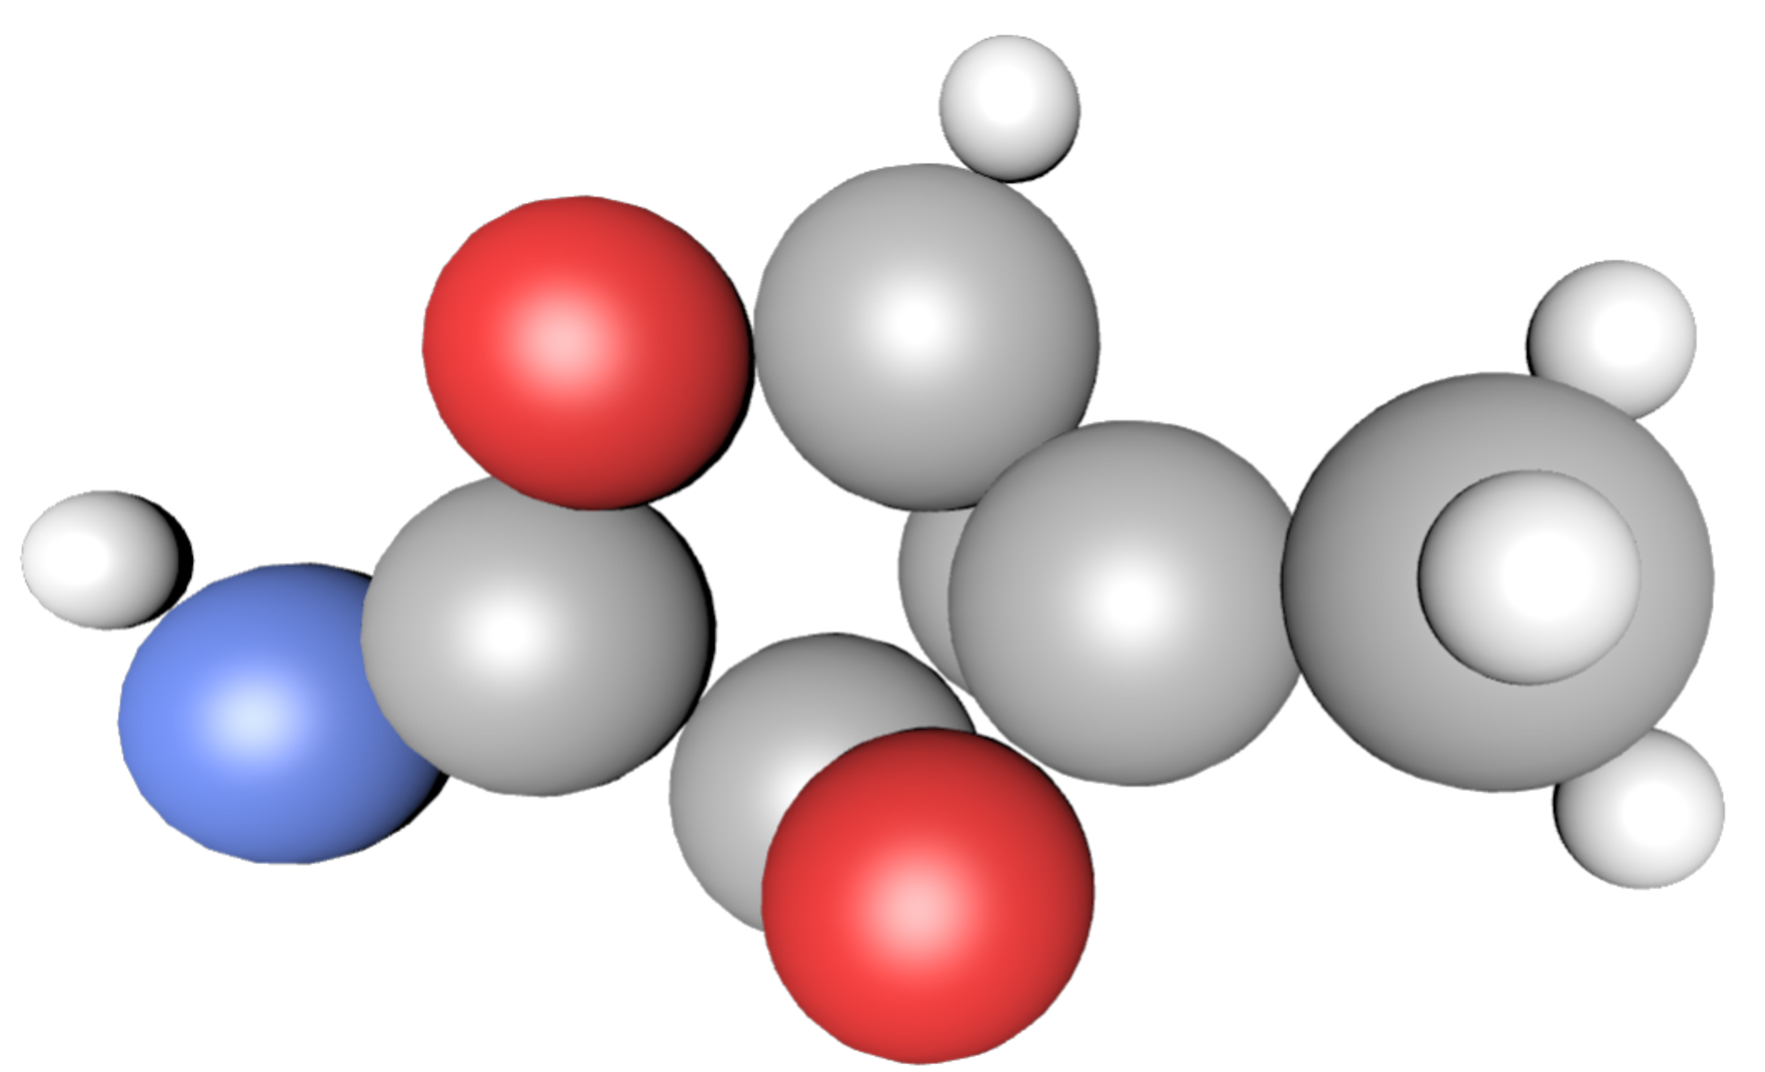
\includegraphics[width=\linewidth]{figures/molecule-3d-1}
	\caption{A 3D structure of a small organic molecule. Carbon and hydrogen atoms are shown in gray and white, respectively. The red spheres show oxygen atoms and the blue one shows a nitrogen atom according to the common coloring convention. In size of the spheres is chosen such atoms that covalently bonded atoms have no or almost no space between them. 
	}
	\label{fig:molecule-3d}
\end{figure}

When it comes to 3D structures there are really only two basic ways of representing them modeling with DNNs. The first is to describe them as 3D grids and using 3D convolutional networks simply extending the same architectures used in computer vision by an additional dimension~\cite{Wallach2015}. In this approach, you would literally use the the 3D color image shown in Figure~\ref{fig:molecule-3d} as model input. The problem with this approach is two-fold: First of all, the cubic number of data-points make this method computationally very expensive. The second problem is that the information encoded in all these data-points is highly redundant. In molecular structures, coordinates and types of atoms are fully sufficient to describe the molecule. All other information - such as atomic radius, etc. - are functions of the types of atoms (hydrogen, carbon, etc.). Thus when for instance a ten-atom molecule is fully described by ten coordinate vectors and ten atom types (40 numbers), it is excessive and inefficient to model it as a 3D image with tens or hundreds of thousands of pixels. The advantage of the 3D convolutional approach is that 3D structure information is necessarily provided to the model which is a challenge for MPNNs as explained in the next Section~\ref{sec:limitations}.



The idea of using graphs to model molecules comes quite naturally when looking at the most common way of representing small molecules in text books: so called molecule graphs such as the one shown in Figure~\ref{fig:caffeine}. A molecule is usually defined as a number of atoms connected by covalent bonds. These kind of bonds involve the sharing of one or more electron-pairs between the bonded atoms and chemically very stable - i.e. it takes considerable energy or the involvement of enzymes to break them up~\cite{Organic-chemistry}. In laymen's terms, covalent bonds can be regarded as 'stable under normal conditions'. In the commonly used molecule graph representation, atoms are shown as letters denoting their type and the covalent bonds are drawn as edges between them as shown in Figure~\ref{fig:caffeine}. Thus defining a graph where atoms are the nodes and covalent bonds are the edges seems like the most natural way of modeling molecules. However, upon closer examination, the situation is somewhat more complicated.


\begin{figure}[H]
	\centering
	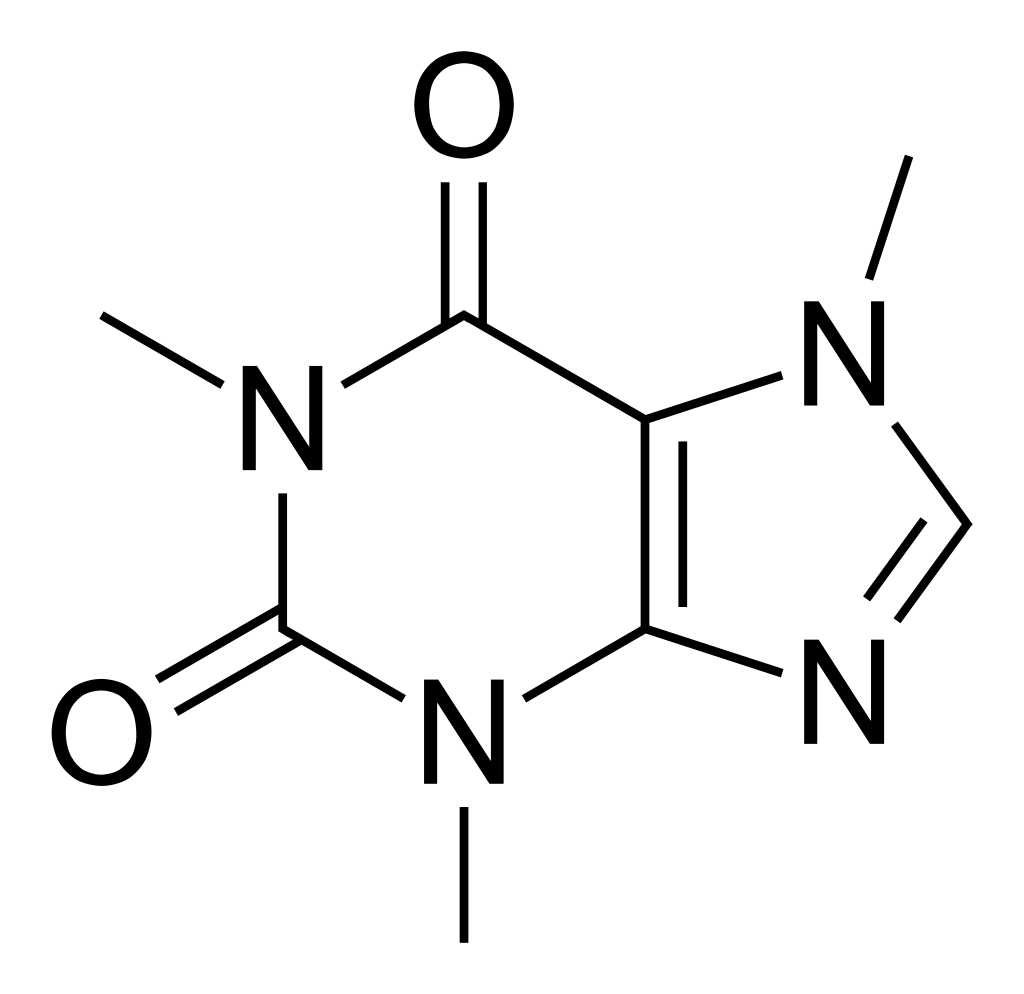
\includegraphics[width=0.7\linewidth]{figures/caffeine}
	\caption{The standard molecule graph representation of caffeine which was consumed in large amounts during the writing of this thesis is shown above. The lines represent edges in the graph. Line intersections or end-points show atoms which represent nodes in the graph. Most of these atoms are carbon atoms as in (almost) all organic molecules which are not indicated by a letter in the molecule graph - instead every line intersection or endpoint without a letter represents a carbon atom. Other heavy atoms are denoted by their single letter code such as Oxygen an Nitrogen shown as O and N, respectively.
	By convention, hydrogen atoms are not drawn at all because their presence can be deduced from the information shown and is thus redundant. (For instance the carbon atom represented by the bottom-most line endpoint has three hydrogen atoms attached to it. That can be deduced form the fact that each carbon atom engages in four bonds with other atoms. As the only one such bond is shown as the edge between the bottom-most carbon and the bottom-most nitrogen atom, three are left. These are assumed to be occupied by hydrogen atoms by convention if they are not drawn explicitly. These considerations become relevant when trying to omit hydrogen atoms from the input data as described in Section~\ref{sec:no-hydrogens}.)
	Furthermore, double- and triple-bonds are shown in such graphs as two or three lines between two atoms. These bonds are stronger and the distance between the atoms is shorter than in the case of single bonds~\cite{Organic-chemistry}. In the graph representation, these types of bonds are represented as edge-attributes because there is no such thing as several edges between any two nodes in a graph. Instead, every edge has a categorical feature bond-type which can be either singe, double or triple.
	}
	\label{fig:caffeine}
\end{figure}


Atoms interact not only if they are covalently bonded. There is a wide array of non-covalent interactions that have a large influence on molecular properties or function such as Van der Waals forces (a simple example being positive and negative partial charges)~\cite{Organic-chemistry}. The strength of non-covalent interactions is a function of atom types, distance and the local environment in the 3D structure. Thus, only including covalent bonds leads to considerable loss of information. As an example, consider that two atoms can be close in space and interact non-covalently even though the path length in the covalent graph may be quite large.

With these considerations, another way of representing a molecule as graph would be to simply define an edge between every pair of atoms if the distance is below a certain threshold. Yet another way of constructing a graph from a molecular structure is to draw an edge between any given atom and it's k nearest neighbors.

All approaches that define the presence or absence of edges by certain rules suffer from inductive bias: we decide in advance which relations between nodes in the graph (atoms) are relevant and which are not. Hence the model cannot learn this information from the raw data but is restrained by predefined rules. Ideally, of course, we would prefer to allow the model to learn everything from the raw data only which is the reason behind the success of deep neural networks in other fields. One way to get rid of this inductive bias is to simply add an edge between any two atoms in the molecule - thus creating a complete graph - and add the distance between the atoms as an edge feature. This way, the model can 'decide' whether a relation between two atoms is relevant based on the distance. The disadvantage of this approach is the high computational cost which makes it impossible to apply to large molecules. This trade-off between inductive bias an computational feasibility lies at the core of one of the key experiments in the thesis described in Section~\ref{sec:neighborhood-expansion}.

%Furthermore, the distance could be added as an edge-feature.
%
% along with a binary feature indicating whether the atoms are covalently bonded or not. This representation has the advantage of considering non-covalent interactions but also introduces many more edges which increases the computational workload.

These examples highlight an importance difference between the theory of MPNNs and their application. In the theory, the starting point is graph structured data and all the effort goes into construction the best possible model architecture to extraction information from this data. For practical application, the data has to be modeled as graphs in a way that captures the available information in the best possible manner. The choices made in this process may have more influence on the quality of the predictions than the choice of MPNN architecture. After all, if incomplete information is fed into the model, even the best model will yield disappointing results. In the next section, we will examine some challenges that arise modeling molecules as graphs for MPNNs.


\subsection{Limitations of Graph convolutional neural networks for molecular structures}
\label{sec:limitations}

\subsubsection{Lack of 3D structure representation}
\label{sec:lack-of-3d-structure}

In principle, 3D coordinates could simply be added to the node features to obtain a 3D graph. However, this is not meaningful for representing 3D molecular structures. First of all, there is no logical reference point for the origin of the coordinate system. The molecule can be translated arbitrarily along one, two or all three spacial axes without changing anything of relevance. The second problem is, that molecules have no natural orientations i.e. they can be arbitrarily rotated where every rotation is just as valid as any other one (in contrast to everyday objects, such as cupboards or cars, where certain rotations are unlikely to be encountered in everyday life). Figure~\ref{fig:rotation} shows two randomly chosen rotations of a small organic molecule. While two images represent the exact same information, the actual atom coordinates are completely different.

\begin{figure}[H]
	\centering
	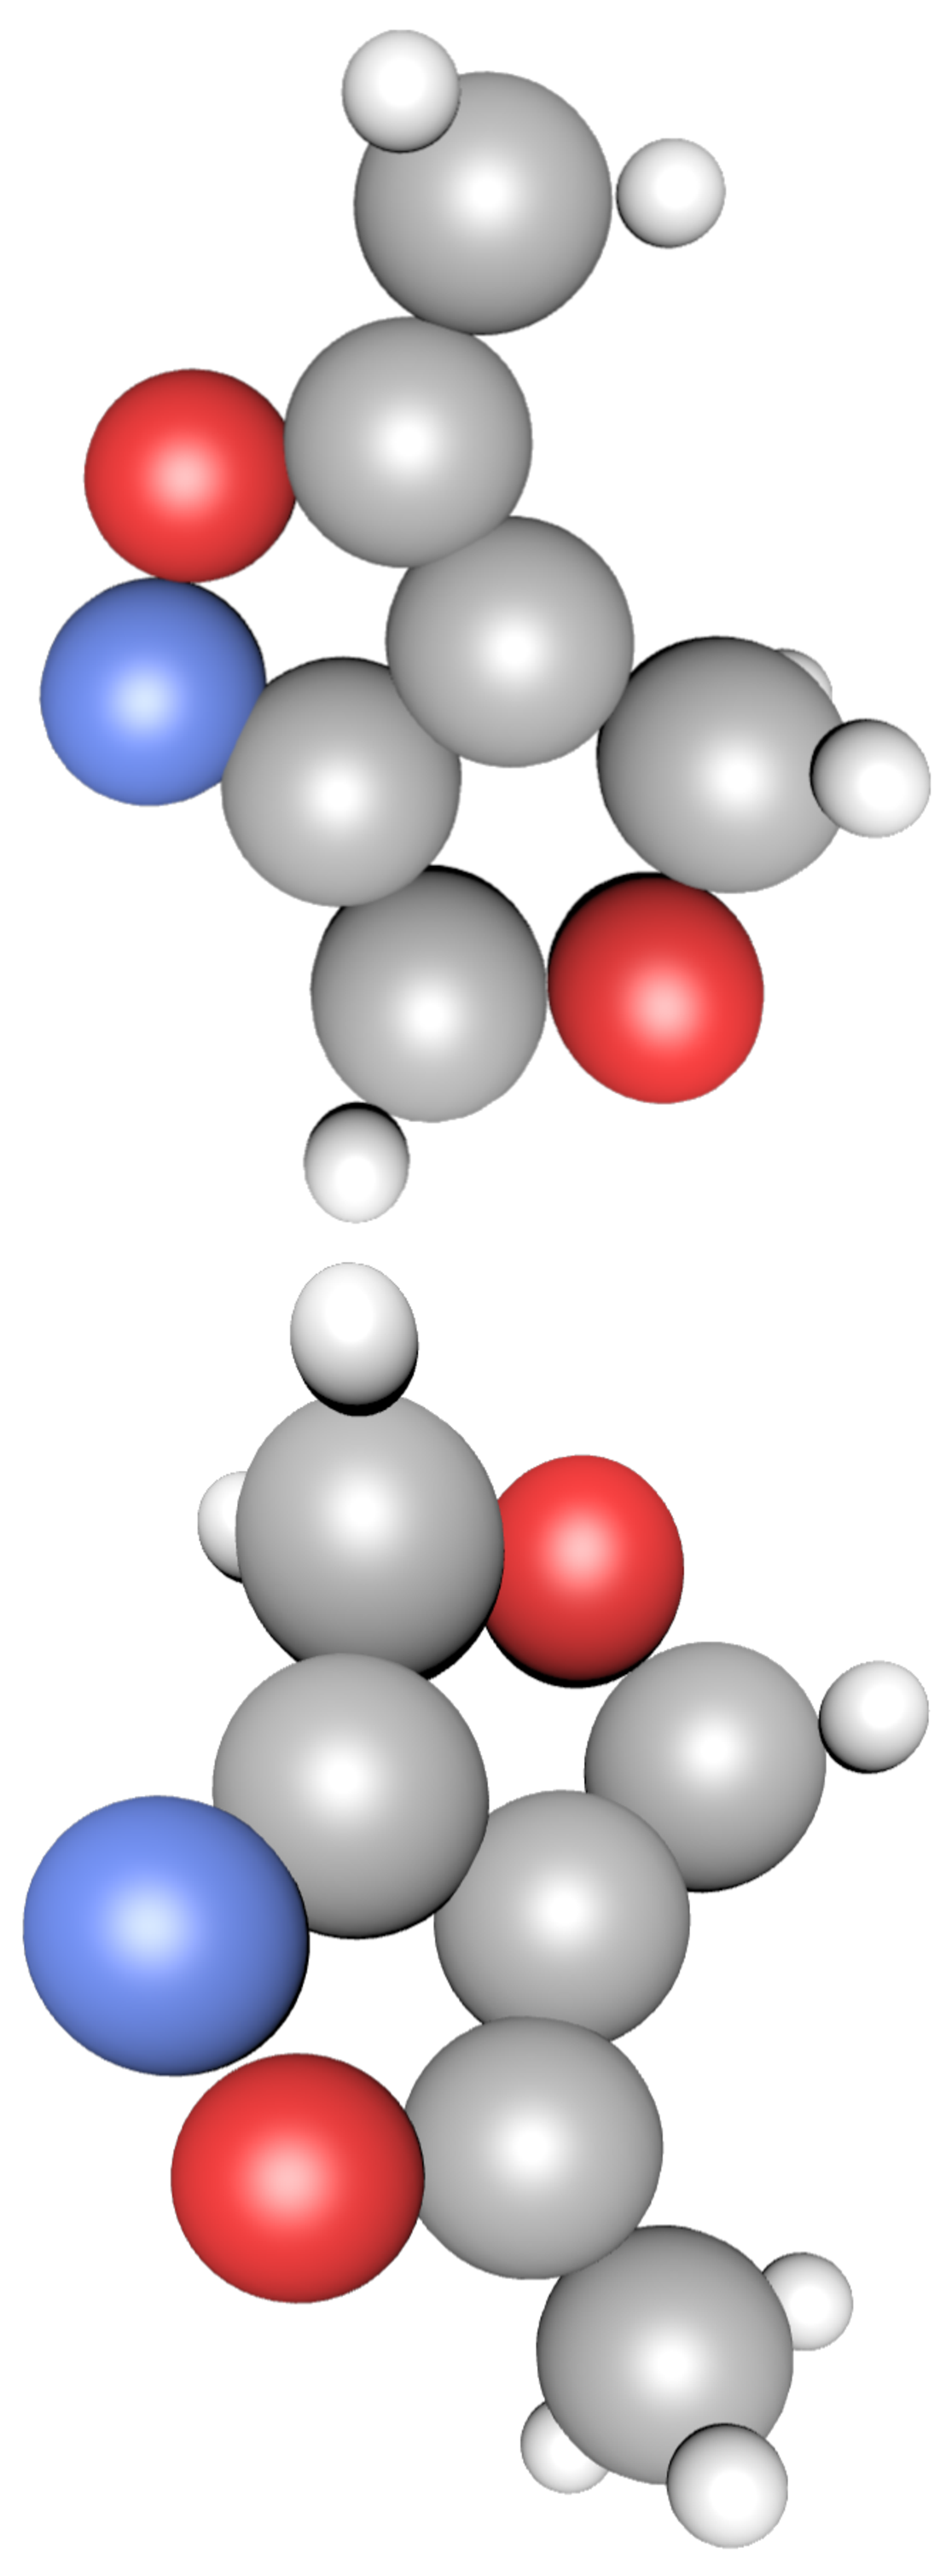
\includegraphics[angle=270, width=\linewidth]{figures/rotation}
	\caption{Two randomly chosen rotations of the same molecule. The values of the atom coordinates are completely different between the two rotations even though the underlying information is the same.}
	\label{fig:rotation}
\end{figure}

For these reasons, the concrete values of the 3D coordinates which depend on this arbitrary positioning and rotation of the coordinate system do not posses relevant information as such. The translation issue could be addressed by instead using directional vectors from one atom to another as edge-features. These vectors are invariant to the arbitrary translation of the molecule in the coordinate system. However, they depend on the arbitrary rotation of the molecule rendering them also not useful to encode the 3D structure as shown in the experiment of Section~\ref{sec:direction-vectors}.

In most MPNN architectures, the euclidean distance is provided as an edge feature. This encodes part of the 3D structure in the graph but still looses vital information. Consider for instance the case of the neighborhood of the the blue nitrogen atom in Figure~\ref{fig:rotation}. The set of distances to the other atoms is unambiguously derived from the 3D structure (irrespective of the rotation). However, only by knowing the distance to each other atom in the molecule the structure cannot be derived. There could be a completely different structure giving rise to the same set of distances. For instance, the fact that the blue nitrogen atom is at the margin of the molecule and not in the center is not contained in the information provided by the distances to all other atoms.

%It is straightforward to see that for most graphs with distance as edge feature, there are many 3D structures satisfying these constraints. In other words the mapping from 3D structure to graph with distances is unambiguous but the inverse operation is not.

It does not take much chemical expertise to conjecture that not providing the full 3D structural information to the model limits it's capability to make accurate predictions. However, there is no easy way to avoid this dilemma and to my knowledge, no satisfying solution has been found so far.

\subsubsection{No down-sampling during feature extraction}

In computer vision with regular CNNs, feature maps are down-sampled to a lower dimension (while expanding the number of channels) every few layers. It makes perfect sense, that higher-level features correspond to larger parts of the original image while at the same time requiring more channels to represent the information. Intuitively, one can think of a data-point on a feature map close to the end of the convolutional part as containing features that summarize a larger region of the original image. The connection between higher-level features and lower dimension feature maps is so central to regular CNNs that it is hard to imagine it any other way. However, no analogous process exists in MPNNs.

In MPNNs, the higher-level features (i.e. the node hidden states) are always associated to their respective nodes throughout all graph convolutional layers. While each of the node hidden states contains information from the node's environment, there is no representation that summarizes a whole group of nodes. However, after the graph convolutional layers, all the node representations are immediately aggregated to give a graph representation.

In the example of molecules such down-sampled representations could represent groups of atoms instead of just individual atoms. In organic chemistry, there are is a limited number of chemical groups that appear frequently in organic molecules and strongly determine their properties and function called functional groups. Many of those functional groups are composed of only three to four atom and appear very frequently in organic molecules (Carbonyl, Hydroxyl, Amide, Amines, etc.)~\cite{Organic-chemistry}. A model with the ability do down-sample would likely learn representations of these important functional groups. Another benefit of such a mechanism would be to feed angle-information into the model. Note that angles are neither node- nor edge-features. Instead, an angle is a property of a group of three nodes (or you can also see it as a property of a pair of edges). Having a representation for a group of - for example three - nodes would allow to add the angle as a feature thus providing more structural information than only distances.

For these reasons it is my strong believe that future successful MPNN architectures will likely have some sort of down-sampling mechanism that allows learning representations for groups of nodes.




\chapter{Methods, data and evaluation}
\label{chapter:Methods}

%describe in detail architecture of the tencent MPNN and its variants, optionally discuss the code explain where the code is found and how to run it

\subsection{Data and features}

The new quantum chemistry dataset \textit{Alchemy}, created by Tencent Quantum Lab, was used for this thesis~\cite{Chen2019}. The dataset is similar to the well established QM9 dataset with the same quantum mechanical properties available and a similar number of molecules. The main advantage of the new \textit{Alchemy} dataset is that it also contains larger molecules of up to 14 heavy atoms (i.e. non-hydrogen atoms) as opposed to the maximum of nine heavy atoms in the Q9 dataset.

There 119487 molecules in the dataset containing the 3D coordinates for each atom, its type and the information which atoms are covalently bonded and with which bond type and twelve important quantum mechanical properties~\cite{Chen2019}. The task is to predict these twelve properties from the raw data.

There are two different approaches to go about this task. The pure deep learning approach is to use only coordinates and bonds and rely on the network to learn to extract any features required to predict the target properties. After all, coordinates, atom types and bonds contain all the available information (actually the bonds could be reliably calculated from coordinates and atom types and thus, strictly speaking are redundant information).

The other approach is to calculate all sorts of chemical features using open source python libraries and feed them in to the model alongside the raw data. Such features are node (atom) features (whether the atom is an electron donor or acceptor, whether it is an an aromatic ring, it's hybridization type, etc.) as well as bond (edge) features. The fact that these features are calculated from the raw data without any additional information means that the model should also be able to learn to compute them if required. Hence, calculating features and feeding them into the model should in theory be obsolete but could give a slight performance boost if the model would not be able to learn those features. Since the focus of this thesis is deep-learning, no manual feature computation is performed here except if it is required to allow comparison with results from the literature.

% explain target properties


\subsection{Base network architecture}



\subsection{Training}

% optimzer, lr, etc.

\subsection{Benchmark and evaluation}


\subsection{Experiments}



\chapter{Results}
\label{chapter:Results}


\section{Using graph convolution in the way it's meant to be used gives poor results on molecular structures}

In the paper Chen et al.~\cite{Chen2019} at Tencent Lab, the authors modify a well performing GCNN architecture for quantum chemistry invented by Gilmer et al.~\cite{Gilmer2017}. The authors expand this model by using both, categorical bond type and euclidean distance as edge features and observe considerably better performance. At first glance, the use of both kinds of features - which seems to be implied in the paper - looks like a plausible explanation for the success. However, a upon closer inspection, the reasoning does not add up. Bond types almost completely determine the euclidean distance. E.g. ever carbon-carbon single bond has a distance of []Å, every carbon-oxygen double bond is []Å long, etc. [CITATON]. (The same applies to the reverse: knowing the distance between two atoms as well as the atom types allows to deduce the type of covalent bond or lack thereof.) Therefore no additional information is added by including the euclidean distance as a feature. Inspection of the implementation reveals anther possible reason for the good performance of the Tencent Lab-paper is quickly identified: Not only is the euclidean distance added as a feature to existing edges, every atom is connected to every other atom in the molecule with the euclidean distance being the only not-null feature~\footnote{\url{https://github.com/tencent-alchemy/Alchemy}}. Thus, the structure of the graph is changed dramatically form the graph of covalent bonds to complete graph where every node is connected to every other node. The complete graph is a special case of graph and is rather untypical because in most applications, the presence or absence of an edge between two nodes is the most important kind of information. Simply connecting all nodes with each other seems to diminish this information (although in this case, the euclidean distance allows to distinguish between important and less important edges). With these considerations it is surprising but very interesting that the approach of Tencent Labs works so well.

In preparation for this thesis, I participated in the Tencent-Alchemy competition~\footnote{\url{https://alchemy.tencent.com}} using approach described above a baseline architecture. Despite many experiments, I achieved the best results simply fine-tuning Tencent Labs model and finished 26th out of 53 participants. The fact that half the participants did not beat the baseline published in the official competition paper, shows that the approach is indeed quite effective an warrants a closer examination why the peculiar approach of using complete graphs works quite well.

%As discussed in the introduction, a central concept of graph convolution (and regular convolution as well), is to compute a representation of a local neighborhood. In the case of graphs, a local neighborhood is a node and its neighbor nodes while on images, it is a small patch of pixels, such as 3x3 or 5x5.


As explained in the introduction, we can define the neighborhood of a node as all other nodes within a certain distance threshold. We refer to this threshold as neighborhood radius.

Therefore, the first experiment, we compare the learning curves of graphs when defining the neighborhood with different thresholds. First of all, covalent bonds are always represented as edges in the graph. Then, for increasing radii, edges to all non-covalently bonded atoms within the radius are added to the graph. A neighborhood radius of zero thus means that no additional edges are added to the graph - the graph only has edges between covalently bonded atoms. At a radius of 1.5 Ångström (1Å = 10nm), an edge is added between any two non-covalently bonded atoms with a distance of at most 1.5Å. The same is done for 2Å, etc. For perspective, most covalent bonds in organic molecules have a distance of around 1Å [CITATION]. 1.5Å is very close for non-covalently bonded atoms such that only very few non-covalently bonded atoms - if any - will be within 1.5Å of an atom in an organic molecule. With a 2Å radius, every atom in the molecule will get some new neighbors due to this rule. With a 4Å radius, many atoms will be included in the neighborhood that have very little to no interaction with the central atom. At 5Å, for many small molecules, every atom is considered a neighbor of any other atom - applying this radius is therefore similar to connecting every atom with every other atom in the molecule. Finally, with an infinite radius, a complete graph is obtained.

\begin{figure}[H]
	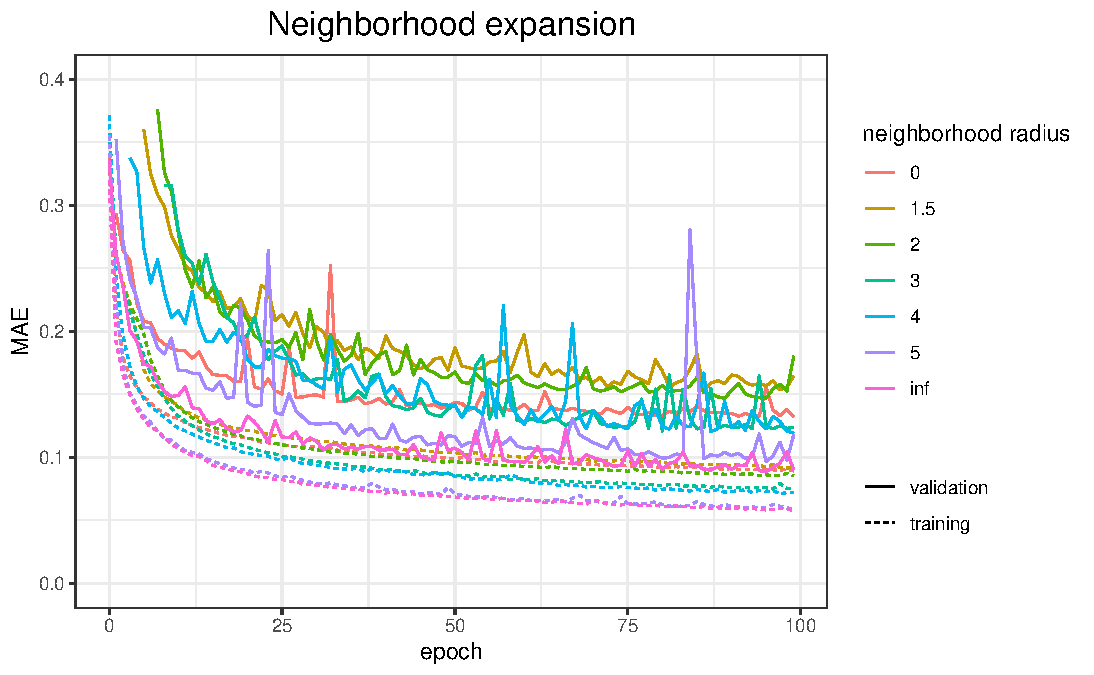
\includegraphics[width=\linewidth]{figures/tencent-mpnn-neighborhood-expansion}
	
	\caption{The learning curves with different neighborhood radii are show over the courses of 100 epochs. The color corresponds to the neighborhood radius, dotted lines the training errors and solid lines show validation errors. Note that for each radius, there is a training- and a validation-error curve. Each curve is an average of three learning curves with the same neighborhood radius. All curves were generated using a simple optimization scheme described in Section~\ref{sec:training}. Both, validation- and training-error could be lowered considerably by employing a more sophisticated optimization scheme. However, this would be at the expense of comparability between curves.[REFERENCE]}
	\label{fig:tencent-mpnn-neighborhood-expansion}
\end{figure}

As Figure~\ref{fig:tencent-mpnn-neighborhood-expansion} shows, the best performance is indeed achieved with the complete graph - connecting every atom with every other atom in the molecule with an edge. In general, the larger the neighborhood radius, the better the performance~\footnote{Exception: radius 0}. This result is in line with the suspicion that the real reason for the good performance of Tencent Lab's model is the addition of new edges rather than the addition of the euclidean distance feature.
The result is somewhat counterintuitive and in contrast with the principle of (graph-)convolution. As described in the introduction, in theory, graph convolutions update node-representation based on the local neighborhood of each node. Eventually, after $t$ layers, each node representation would contain indirect contributions from all other nodes with $t$ or less edges between. However, the results shown here show that the performance is best if the graph convolution considers all atoms at every layer. This contrast clearly shows that much remains to be discovered about the use of GCNN for molecules.

For small molecules and with considerable computational power at hand, one could simply accept this finding as it is and represent molecules as complete graphs. However, for larger molecules with hundreds of atoms, this would be computationally not feasible as the number of edges increased quadratically ($\frac{n(n - 1)}{2}$ edges for $n$ nodes). Therefore, further experiments will aim at finding an alternative way that captures the advantage of the complete graph-approach without the excessively high computational cost.


%Show that, for decreasing thresholds, performance decreases
%
%Emphasize that this is not really appreciated in the literature.
%Cite Alchemy paper and point out that the high-performing kaggle-teams all use fully connected graphs.
%Does no one notice?
%
%Repeat that the conv should be able to handle this because after several MP steps, the effective field of vision is the entire molecule - but it doesn't work well


\section{Manual feature engineering does not improve prediction accuracy.}

% compare raw vs. tencent features.
% after the point has been made, use only raw data

\section{Excluding hydrogen atoms from the molecule-graph speeds up training but reduces prediction accuracy}

Another possible preprocessing step is to disregard hydrogen atoms and instead add the number of hydrogen atoms bonded to a given heavy atom as a node feature. The rational behind this step is that the properties chemical properties of hydrogen atoms depend strongly on the heavy atom to which it is bound. While some information is lost during this step, the number of atoms in the molecule is reduced by an average factor of [CHECK value]. This modest reduction in the number of nodes leads to a very dramatic reduction in the number of edges. Naturally, this effect is most pronounced in complete graphs where the number of edges increases quadratically with the number of nodes ($\frac{n(n - 1)}{2}$ edges for $n$ nodes). While the average number of edges using complete graphs is [CHECK value] in the AlChemy dataset, this number drops to [CHECK value] after excluding hydrogen atoms.

The approach of not considering hydrogen atoms explicitly but only as features of heavy atoms is known as using \textit{implicit hydrogen atoms}. In short, it is a way of summarizing raw data which speeds up training considerably while loosing some information. Figure [] shows...

% probably: larger error
% => use explicit hydrogen atoms from now on


\section{Introducing a graph-state at every graph-conv layer improves results}



{\itshape
explain hypothesis:
lack of information of global environment. Maybe graph-level features needed at every conv?

Test this hypothesis:
add graph-state
show figure: now the effect is less pronounced because the global environment is accessible through the graph-state

Why this is important:
in larger graphs the option of using a fully connected graph is simply not there:
show computational complexity graph
}


\section{graph-conv layers with independent weights do not improve results}

{\itshape
	
OPTIONAL SECTION

It's reasonable to assume, that different layers need different feature extraction properties (low vs. high level features). In cv, the layers don't share weights.

However, in experiments, the weight-shared graph layers prove superior.
}

\section{relative position edge features improve results slightly}

{\itshape
 Show that relative position edge features slightly improve the results but not much
 
 explain that the problem is probably that they are not rotation-invariant
	
	
OPTIONAL PART:\\
review the results of the 3DGCN-paper and show that this doesn't work really well on the Alchemy data - probably for the same reason given above
}








%\chapter{Discussion}
\label{chapter:Discussion}

\section{First section}

some text...

\chapter{Conclusion}
\label{chapter:Conclusion}

In this master's project, I had the pleasure of investigating the exciting field of Message Passing Neural Networks (MPNNs) for chemical applications. Two different machine learning competitions~\footnote{\url{https://www.kaggle.com/c/champs-scalar-coupling}}~\footnote{\url{https://alchemy.tencent.com}} provided an excellent starting point for experimenting with different data representations and models to predict atomic interactions (Section~\ref{sec:champs}) or molecular properties (Section~\ref{sec:alchemy}). Furthermore, they allowed to benchmark the results against word-class machine learning practitioners and see their fascinating solutions after the competitions.

Graph neural networks are one of the most interesting frontiers of deep learning for a number of reasons. As stated in the Introduction (Section~\ref{sec:motivation}), most of the breakthroughs in deep learning occurred using image-data or natural language data (text and speech). Graph neural networks are one of the most promising methods for extending this success to other kinds of data. Another fascinating aspect of graph neural networks is that their applications encompass a lot of completely different fields from social networks, to documents and molecular structures. For this reason, the model-architectures are also required to be very diverse to fit the different use-cases.

This project investigated the challenges associated with using 3D data in general and molecular structures in particular with MPNNs. We have seen that incorporating 3D structural information into MPNNs in a way that increases the model's predictive power remains a big challenge (Section~\ref{sec:direction-vectors}). Furthermore, the results in this thesis support the pure deep learning approach of only using raw data as model input (Section~\ref{sec:raw-data}). However, the fact that manual feature engineering and raw data are still used alongside each other indicates that deep learning models for chemical applications are not yet as mature and efficient as in other fields (e.g. computer vision and natural language processing) where manual feature engineering has been made completely obsolete by end-to-end differentiable models using raw data only. Therefore, a lot of research remains to be done before MPNNs reach their full potential.

Finally, the project also showed that some of the key factors for the success of a machine learning project are not directly machine learning-related at first sight. One of them is data quality (or the lack thereof) which required a lot of attention in the project at hand (Section~\ref{sec:diff-old-new-ds}). Furthermore, it is vital to make experiments easily reproducible, to be able to run multiple experiments automatically and to store all parameters and results in a systematic manner. To this end, the experimentation-process was largely automated in the project at hand~\footnote{The code is available on github: \url{https://github.com/raph333/masters_project}} and the python library \textit{mlflow} was found to be very useful to store and access all experiment-parameters and results. These factors are even more decisive in large organizations but provide substantial benefits in one-person projects as well.

Summing up, the project was a great learning experience for designing deep neural networks as well as for structuring machine learning projects.

% optional: Appendix with terms and abbreviations

%\input{AppendixA}  % optional: interpreting learning rates (from poi report)

%%%%%%%%%%%%%%%%%%%%%%%%%%%%%%%%%%%%%%%%%%%%%%%%%%%%%%%%%%%%%%%%%
%% BIBLIOGRAPHY.
%%%%%%%%%%%%%%%%%%%%%%%%%%%%%%%%%%%%%%%%%%%%%%%%%%%%%%%%%%%%%%%%%

\clearpage
\phantomsection
\addcontentsline{toc}{chapter}{Bibliography}

\bibliographystyle{IEEEtran} % IEEE bibliographic/citation style.
%\bibliography{IEEEabrv,Thesis}
\bibliography{IEEEfull,Thesis}


\end{document}
